% !TeX root = ../main.tex
% Add the above to each chapter to make compiling the PDF easier in some editors.

\chapter{Implementation}\label{chapter:implementation}
Building on the framework architecture explained in Chapter \ref{chapter:Approach}, we describe Maestro the proof-of-concept (POC) implementation in details to show that the framework architecture is sound. Moreover we describe the flows implementation used to create the experimental use cases to validate elicited requirements in the evaluation chapter.\\

\section{Maestro}


Maestro is implemented as a Java project and web application that act as a middleman between node-RED and SCMAPI. It accepts publish and subscribe requests from node-RED flows through REST API and uses  SCAMPI Java API to propagate these requests to SCAMPI server. Further, whenever it receives a message that it had subscribed to from SCAMPI server, it forwards the message to  node-RED flows who issued the subscription requests. It is divided into several packages, we describe them in alphabetical order:
 \begin{itemize}
 
  \item First, the package \verb|com.middleware.api| which contains two classes, \verb|SCAMPApi.java|  and \verb|MiddlewareApi.java|. The class \verb|SCAMPIApi.java| has a field of type \verb|APP_LIB| from SCAMPI Java API which contains the core methods of SCAMPI server to connect, add status listeners, publish and subscribe to messages.  As shown in Figure \ref{fig:cd-api}, \verb|SCAMPIApi| implements two classes via the \verb|APP_LIB| for the SCAMPI server which includes functions like \verb|OnDisconnected()|, \verb|OnConnectFailed()|,\\  \verb|OnStopped()| and  \verb|OnConnected()|. It also implements \verb|messageReceived()| which handles the messages once they are received from SCAMPI. Further, It contains a cache for messages and a field indicating the machine specification which is read from a file on the device. Also, \verb|SCAMPIApi.java| subscribes to the global identifier of SCAMPI on service initialization which is used as a global identifier for the whole framework. 
 
The class \verb|MiddlewareApi.java| contains REST API for Maestro's web application that runs on port \verb|8080|. It has two requests \verb|POST /publish| and \verb|POST| \verb|/subscribe|  that reference  the \verb|APPL_LIB| in order to submit publish and subscribe requests to SCAMPI server. The class \verb|MiddlewareAPI.java| has a field for the \verb|topicMapping| which is the topic-endpoint mapping we explained in \ref{subsec:send-receieve-data}. Last but no least, it has a main method which in Java is used to run a class. In this case, it is used to run the built  jar file from \textit{Maven} which means once the jar file runs via the command \verb|java -jar interface-1.0-SNAPSHOT.jar|, the main method is only thing that runs and therein it starts a web application via \textit{Spring Boot}.
 \begin{figure}[H]
 	\centering
 	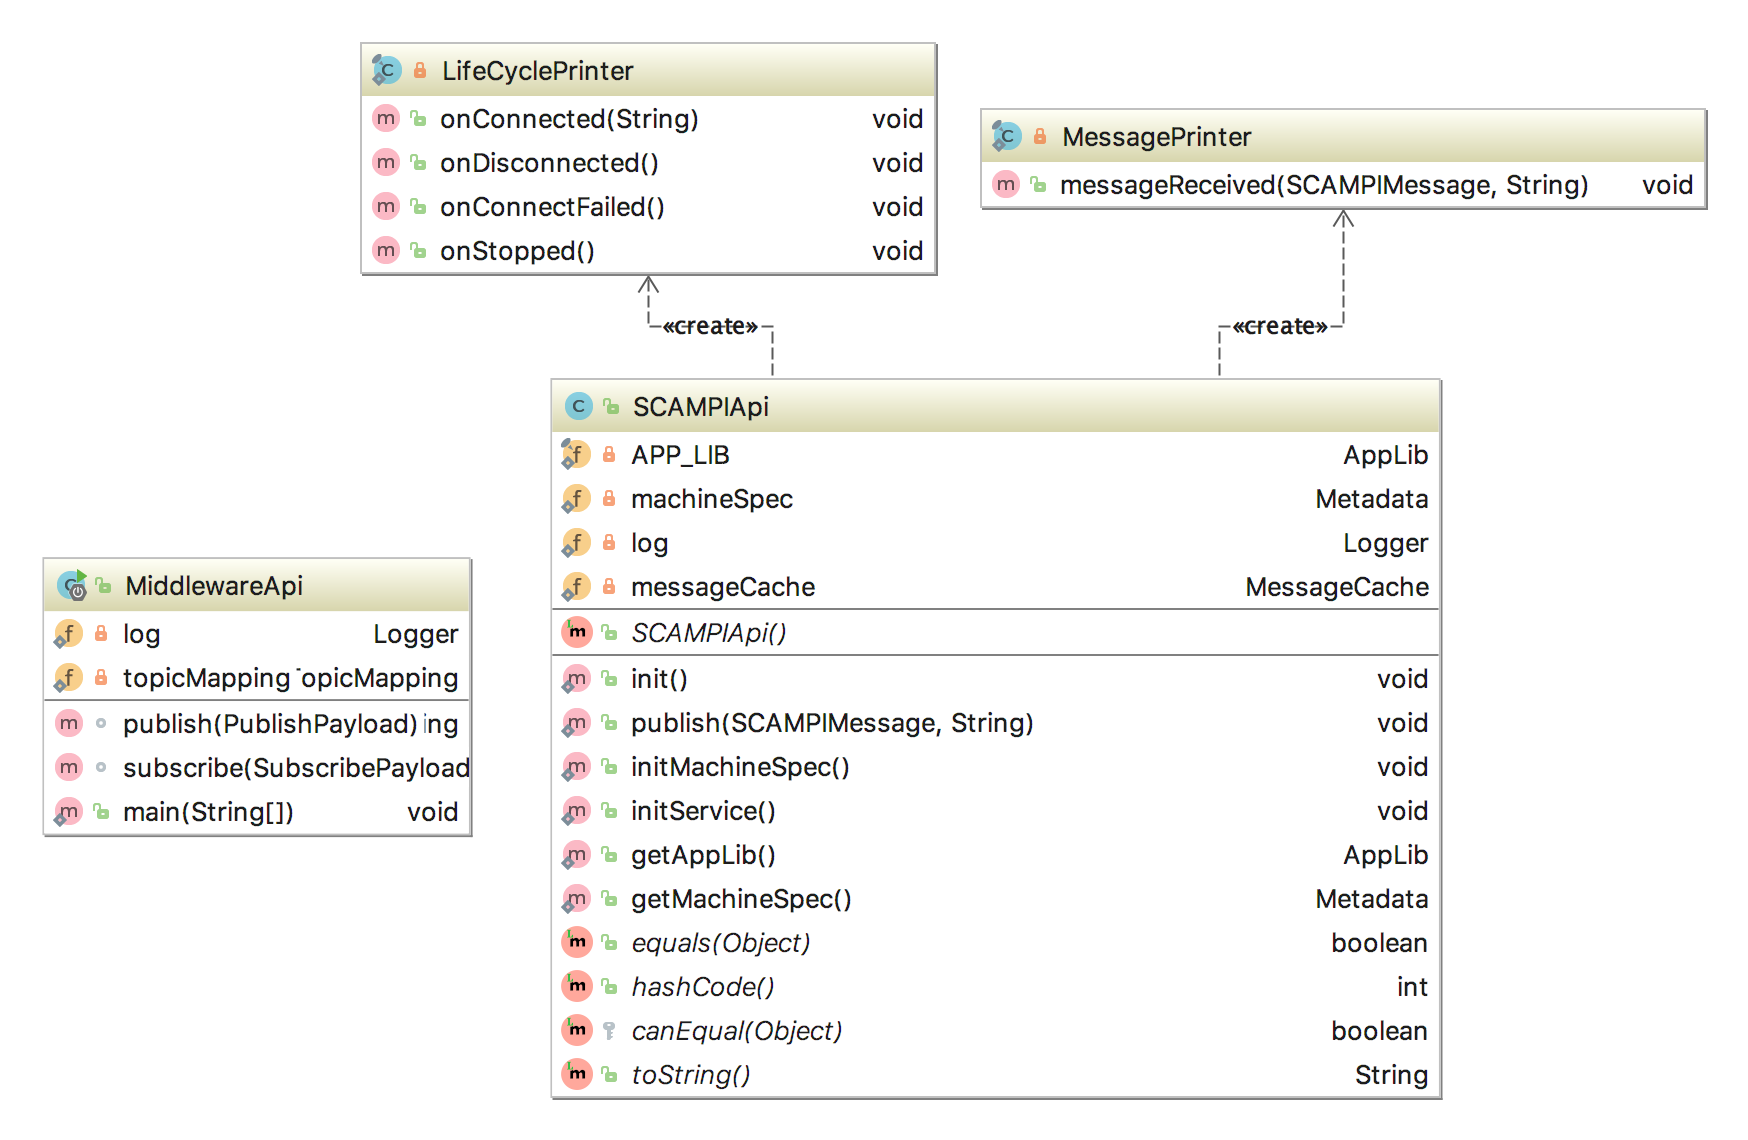
\includegraphics[scale=0.2]{images/cd-api.png}
 	\caption{Class diagram for the api package. }
 	\label{fig:cd-api}
 \end{figure}
 
\item The second package is called \verb|com.middleware.constants| and has one class \verb|Constants.java| which contains all the constant fields used in  Maestro across all other classes. This includes string keys for SCAMPI messages, some Linux commands,  URL for the local node-RED instance, path for user home directory on the hosting machine and path for the JSON file that includes the machine specification. Furthermore, it contains the topic reserved for computations named \textit{Main}. \\
 
 
 \item The third package is the most important one \verb|com.middleware.domain| which contains most of the services that is handled by Maestro. There are two singleton classes namely \verb|ToppicMapping.java| and \verb|MessageCache.java|, the first class is a cache that maps between the subscribed topics and the node-RED endpoints who issued a subscription request to them. The second is a cache that makes sure a received message is not handled more than once. A singleton class means there exist only one instance across the whole web application no matter how long it runs and no other class can create a new instance of these types or re-initialize the existing ones. That's because both are types of caches which should be consistent and global to any class which would need these caches. 
 
 The classes \verb|CommandRunner.java| and \verb|RESTHandler.java| are helpers. The first is used to run commands on the machine and  has two methods \verb|run(String)| and \verb|getFreeRam()| which is equivalent to calling \verb|run("free -m" )|. The second class is used as a REST client for sending requests to node-RED which are used to deploy computations and  send data to endpoints.
 
  Next are the classes \verb|MessageHandler.java| and \verb|Publisher.java| which contain the services for handling incoming messages from SCAMPI and publishing new messages respectively. The \verb|MessageHandler.java| is invoked from  \verb|SCAMPIApi.java| method \verb|messageRecieved()| and differentiates between two types of the messages; computation ones which are received on the topic \textit{Main} and handles them with the method \verb|handleMainTopic(SCAMPIMessage)| that takes care of the resources, machine specifications, puts dependencies on node-RED local directory then the \verb|RESTHandler.java| class is used to deploy the computation to node-RED, and data messages which are received on other topics and handles them with the method \verb|handleSpecialTopic(ScampiMessage)|, it sends the data to any subscribed endpoint in the \verb|toppicMapping| cache using also the \verb|RESTHandler.java|.
 
 The \verb|Pubisher| is responsible for submitting publish requests to the \verb|APP_LIB|. It is invoked from the \verb|MiddlewareApi.java|.  It creates a unique identifier for each new message, and adds the publisher global identifier to the \textit{SCAMPIMessage} as well. It has the same topic differentiation as \verb|MessageHandler.java|.
 On the one hand, if the publish topic is \textit{Main}, it collects the dependencies and attach it to the \textit{SCAMPIMessage} before it sends the message to SCMAPI server. On the other hand, if it is a data topic it checks the attachments and adjusts the response endpoint  to whether it should be sent back to this device only, if this is the case, it creates a mapping between the global identifier of the device and the endpoint that sent the publish request then send it to SCAMPI server. \\
 
 \begin{figure}[H]
 	\centering
 	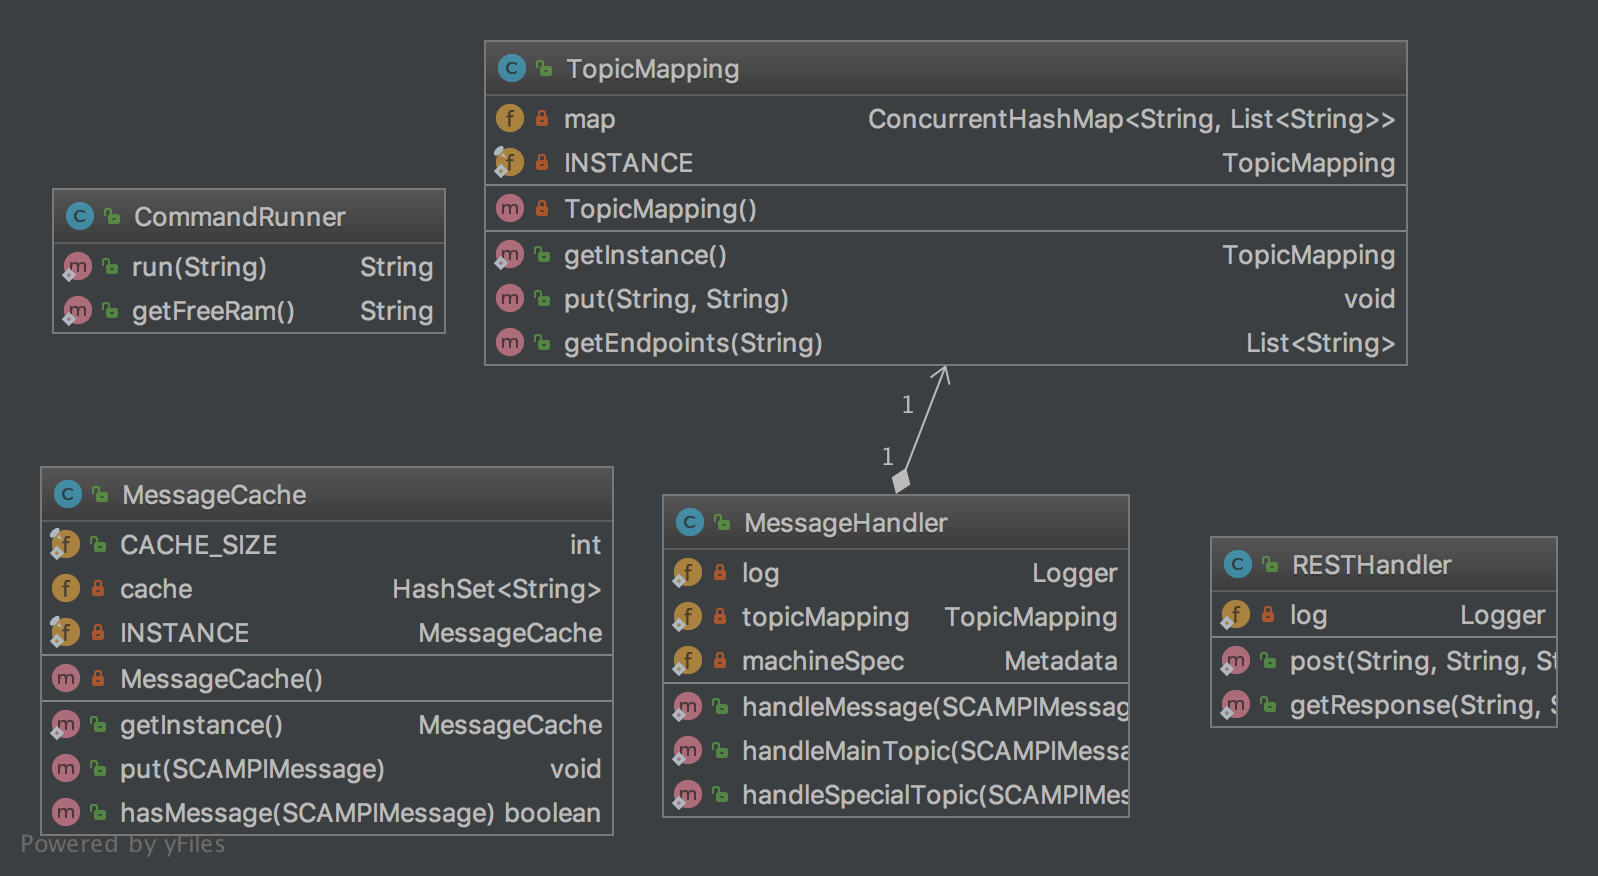
\includegraphics[scale=0.25]{images/cd-domain.png}
 	\caption{Class diagram for the domain package. }
 	\label{fig:cd-domain}
 \end{figure}


\item The fourth package \verb|com.middleware.exception| which contains the project's custom exceptions. Currently it only has a \verb|RESTFailedException.java| class which handles node-RED deployments and data requests failures.

\item The fifth and last package is \verb|com.middleware.model|, it holds the models which are classes used to hold data and encapsulate them. Remark up on that, the Java classes do not contain any getters and setters or constructors. However, using \textit{Lombok} library they are generated in compile time and they can be picked up by the Integrated Development Environment (IDE) as displayed in Figure \ref{fig:cd-models}. 

 \begin{figure}[H]
	\centering
	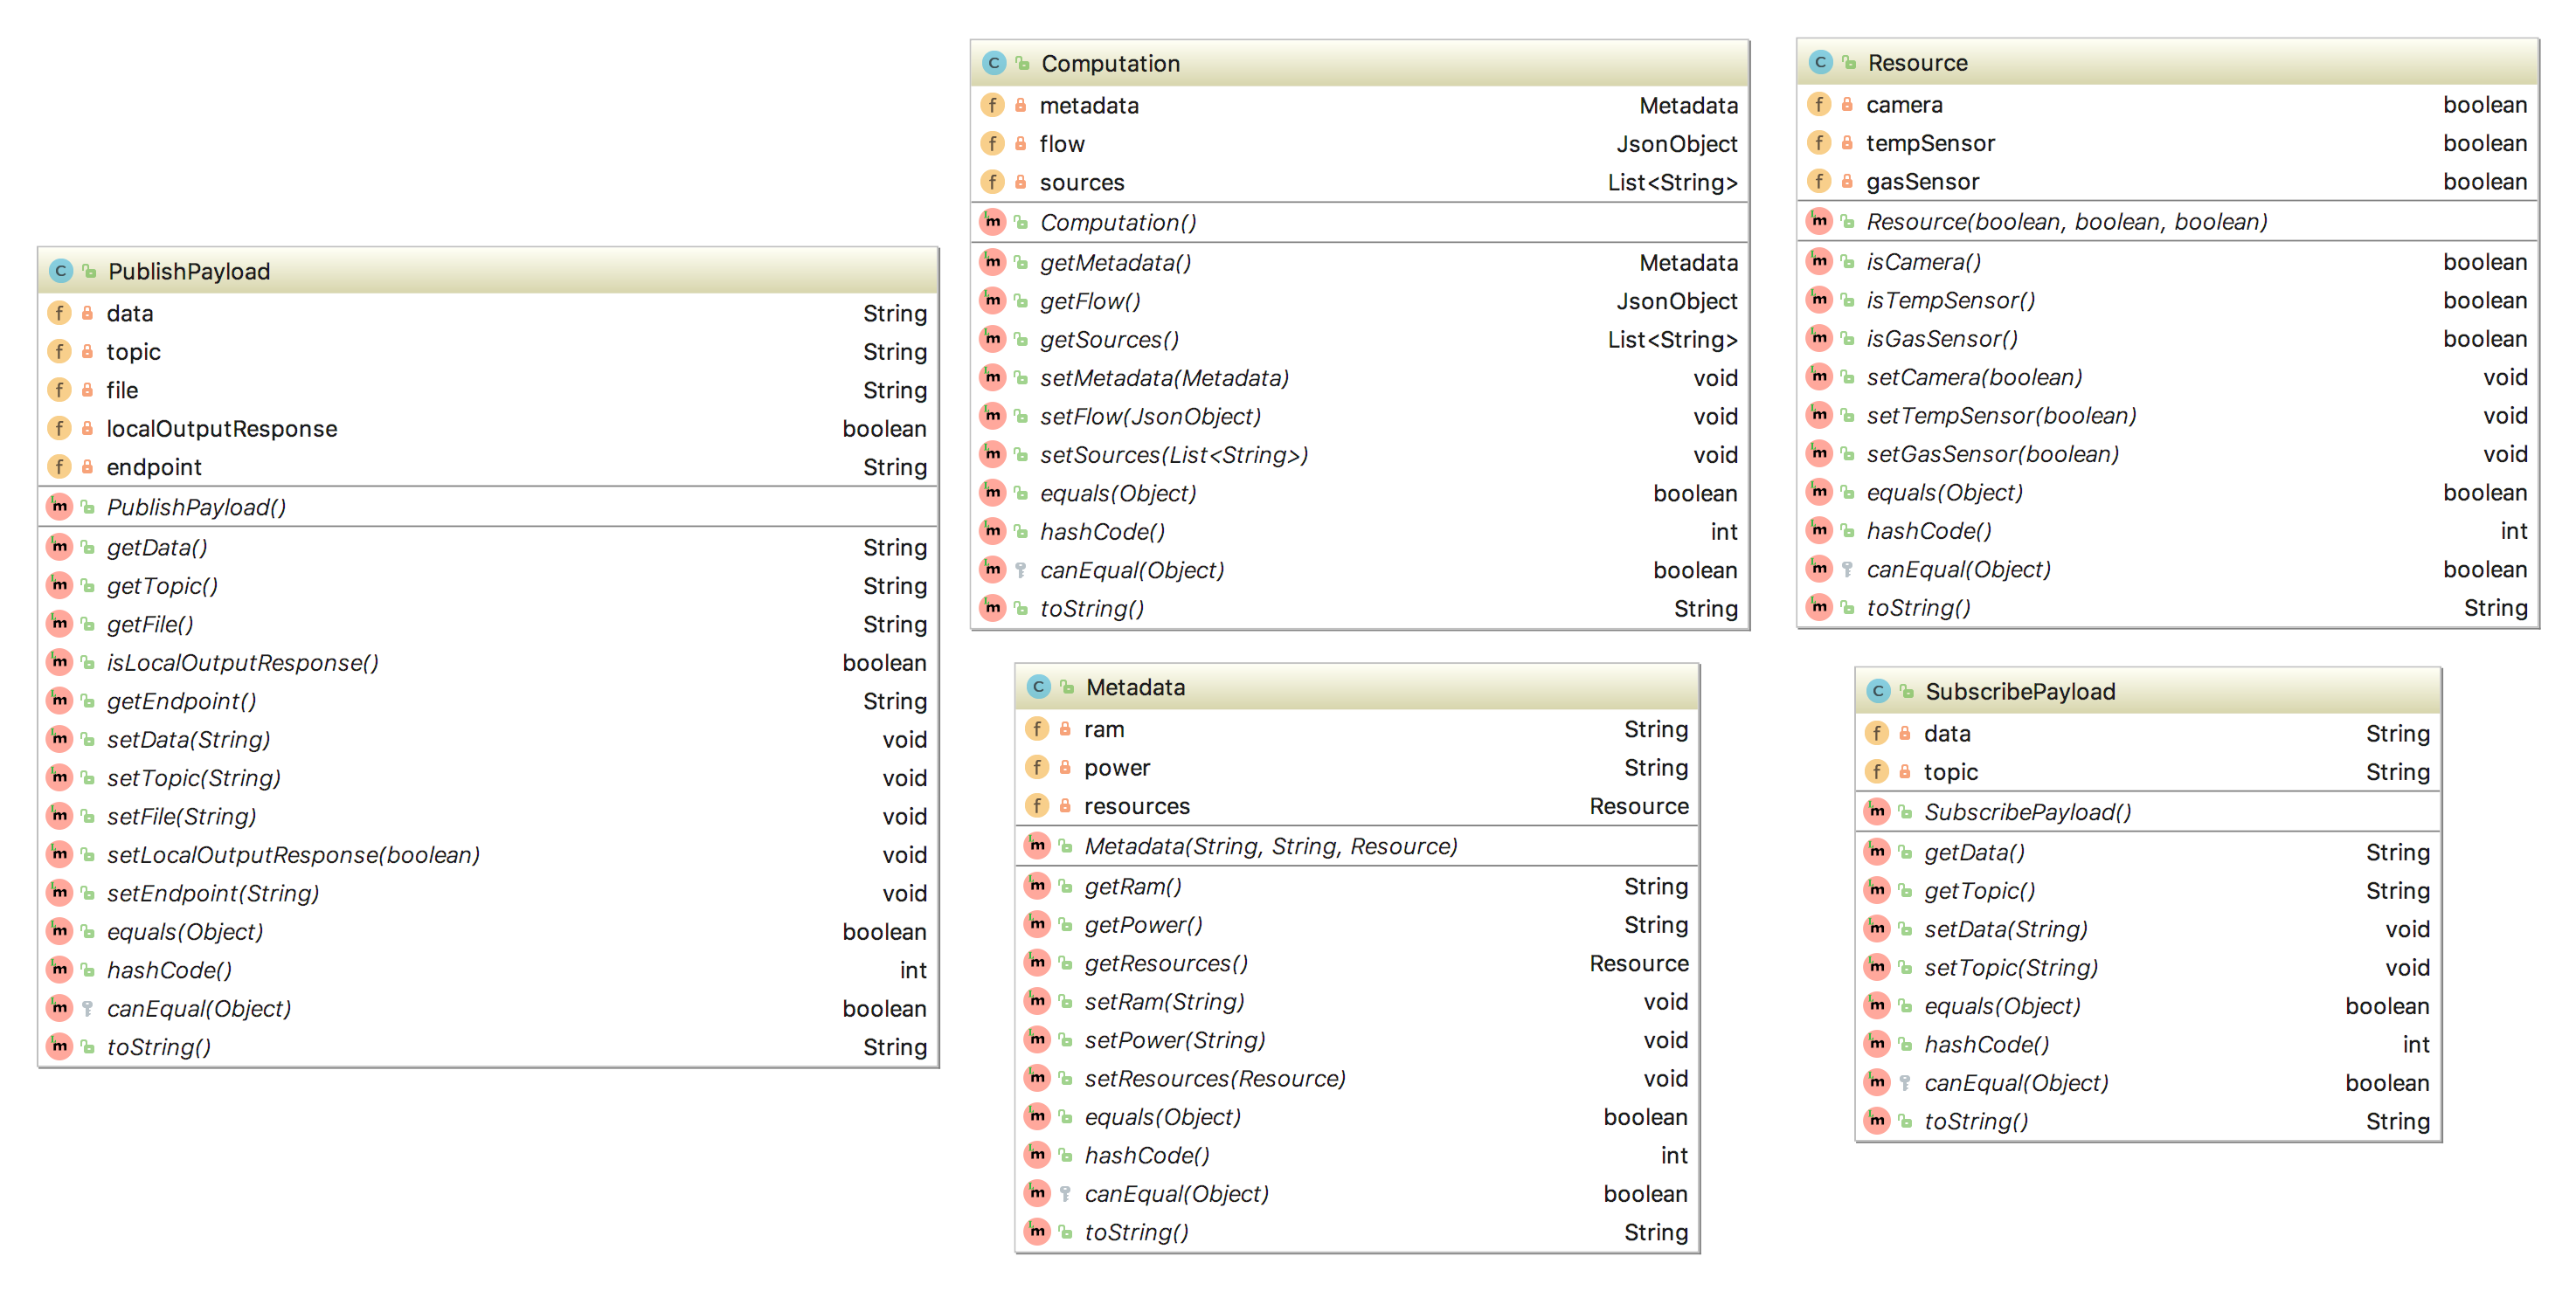
\includegraphics[scale=0.13]{images/cd-models.png}
	\caption{Class diagram for the model package. }
	\label{fig:cd-models}
\end{figure}


\end{itemize}

\noindent Maestro uses \textit{Maven} as a  software project dependency management which handles Maestro's build. \textit{Maven} projects contain a Project Object Model (POM) file which describes the dependencies and libraries used by the project. In addition, it has build configuration management that is used to build the project and create a runnable jar file. Maestro can be compiled and packaged to a jar using the command \verb|mvn clean| \verb|package|. The project contains dependencies for \textit{Lombok} which is a library that generates getters, setters and constructors during compile time without the need to write them in the Java classes, \textit{Gson} dependency in order to be able to read and write in JSON format, \textit{SCAMPI API} which allows us to publish, subscribe and override  functions from SCAMPI and dependencies to create a web application via \textit{Spring Boot}. \\

\section{Flows}
This section explains all the flows developed in this thesis. It shows how the flows can be implemented to achieve different use cases. It also shows how we use node-RED flows in order to send computations.
\subsection{Send Computations}\label{subsec:send-comp}
 \begin{figure}[H]
	\centering
	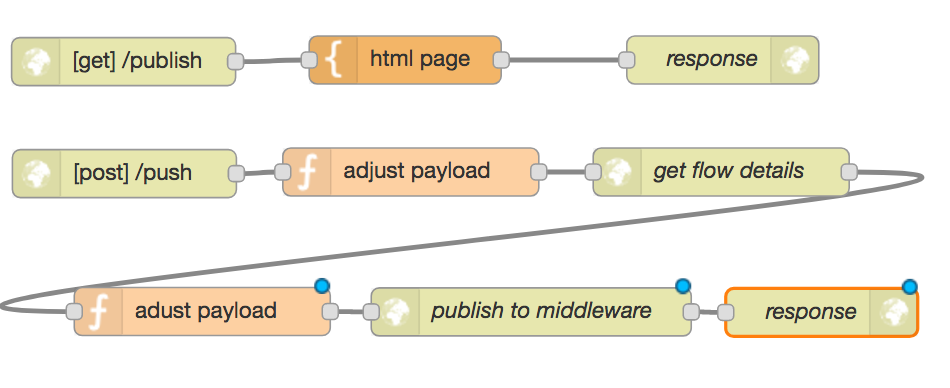
\includegraphics[scale=0.6]{images/flow-publish-computation.png}
	\caption{A flow that publishes computations to Maestro and thus to SCAMPI.}
	\label{fig:flow-publish-computation}
	
\end{figure}

In order to deliver flows which expresses computations for all devices or selected ones according to available resources,  sensors, actuators and also attach dependencies, we developed a node-RED flow shown in Figure \ref{fig:flow-publish-computation}. The flow responds to the endpoint \verb|GET localhost:1880/publish| and returns the HTML page in Figure \ref{fig:html-publish}. Afterwards, the user can adjust the computation power needed by the flow, necessary free Random Access Memory (RAM), sensors and actuators. Then he/she must also write the flow identifier, attach dependencies and eventually click on the button \textit{push} which calls another endpoint on the same flow \verb|localhost:1880/push| with the form data. The endpoint receives the data, fetches the flow details and publish it to  Maestro which handles the rest.


\subsection{Temperature Sensor Alert}\label{susbec:temp}

 \begin{figure}[H]
	\centering
	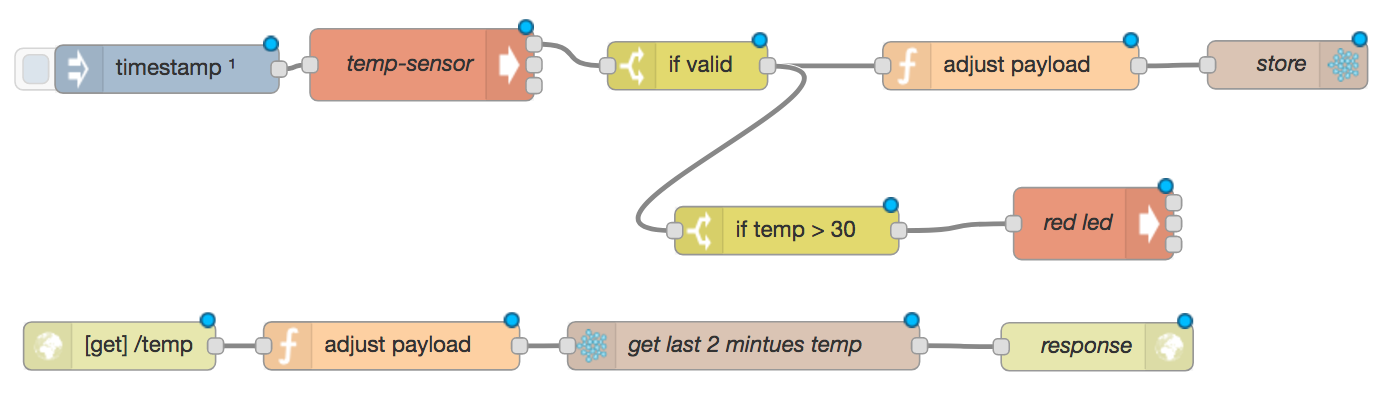
\includegraphics[scale=0.6]{images/flow-temp.png}
	\caption{A flow that reads temperature, stores it and starts a red LED if the temperature is above 30 degree Celsius.}
	\label{fig:flow-temp}
\end{figure}

This flow was developed to make sure that the  framework works against the typical IoT usage of sensors, actuators and time-series databases. As presented in Figure \ref{fig:flow-temp}, the flow runs once it is deployed to any device. Take into account that, it would not have been deployed by Maestro without checking that it has the required resources and dependencies. Once the flow is deployed, it starts a script for sensing temperature  which is sent as a dependency while sending the flow to other devices. It then checks if the temperature is a valid number, then it gets stored in a database. Further, if the temperature is above 30 degree Celsius it runs a script, which is also sent as a dependency, to light up a red LED lamp. On top of that, the flow responds to the endpoint \verb|localhost:1880/temp| and returns all the collected temperature data in the last two minutes.




\subsection{Detect Movement and Store Image Responses} \label{subsec:detect-move}

\begin{figure}[H]
	\centering
	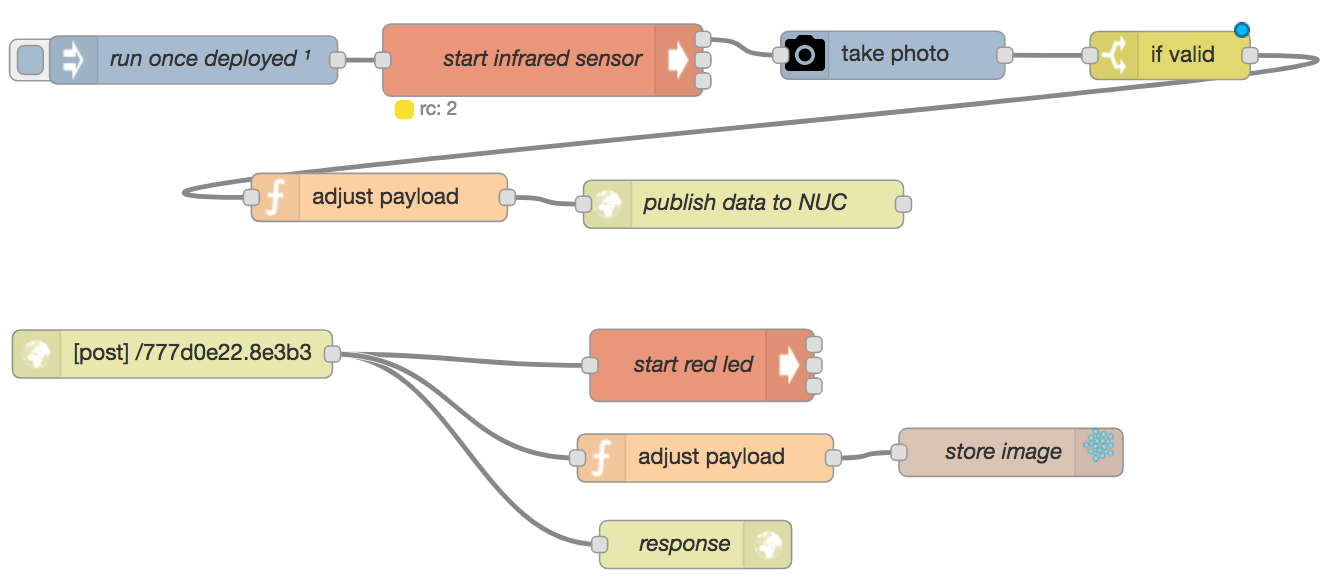
\includegraphics[scale=0.6]{images/flow-motion.png}
	\caption{A flow that detects motion, takes an image then publishes a message and stores incoming responses.}
	\label{fig:flow-motion}
\end{figure}

As part of the implementation evaluation, we developed this flow to take part in a bigger use case. The flow is designed to detect movement through the infrared sensor and then take a picture, which is then published on the topic \textit{NUC} for image recognition. However, in the push payload along with the picture, there is a field stating that the response should come back to this exact device, therefore, Maestro creates a mapping between the device global identifier and the endpoint before publishing. Also, as demonstrated in Figure \ref{fig:flow-motion}, the flow awaits messages on its endpoint and executes a script which starts a red LED, it also stores the recognized image in a database along with its accompanying data. 


\subsection{Show Recognized images}\label{subsec:images}

\begin{figure}[H]
	\centering
	
\includegraphics[scale=0.6]{images/flow-images.png}
	\caption{A flow that creates an endpoint to retrieve stored database images.}
	\label{fig:flow-image}
\end{figure}

Since composability is an important part to validate in our framework. We created a simple flow to show local composable flows. It simply queries the database for recognized images from the previous flow \ref{subsec:detect-move} when requested on the endpoint \verb|GET localhost:1880/images|. It has an HTML page response showing all the images along with their image recognition confidence percentage data and time-stamp. The flow is invoked once it is deployed by the receiving device.


\subsection{TensorFlow Water Bottle Recognition} \label{subsec:tensor}
 \begin{figure}[H]
	\centering
	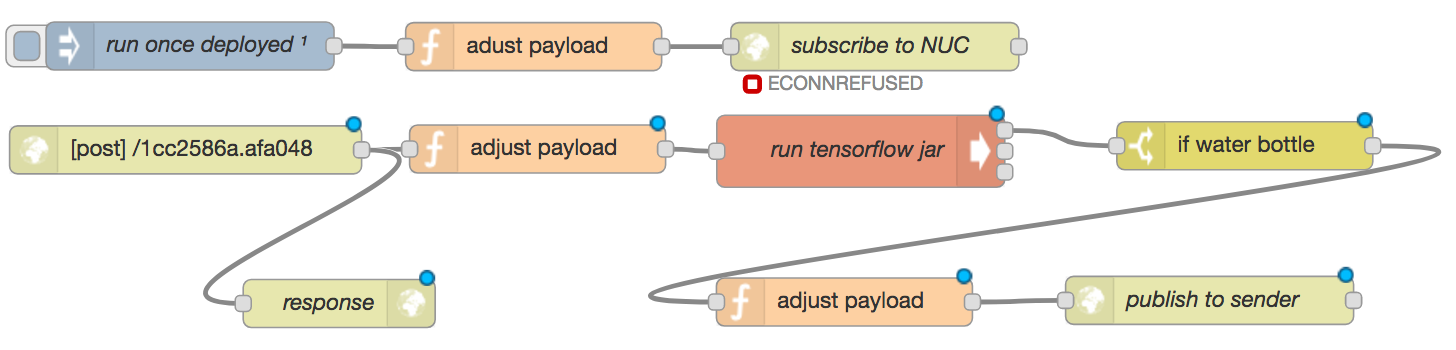
\includegraphics[scale=0.6]{images/flow-tensor.png}
	\caption{A flow that uses tensorflow to recognize a water bottle.}
	\label{fig:flow-tensor}
\end{figure} 

To prove that we can send flows to machines with heavy computation power and lots of free RAM. We developed an image recognition flow using \textit{TensorFlow} which is an open-source software library for machine intelligence. \textit{TensorFlow} needs a 54MB image recognition model that recognizes 1000 object classes, one of them is a water bottle. It also needs the code to run the recognition algorithm which is a Java jar file of 29MB size. Therefore, the flow  needs to carry all the mentioned dependencies. As shown in Figure \ref{fig:flow-tensor}, the flow subscribes to the topic \textit{NUC} once it is deployed. Then, when Maestro instance that runs on the same machine receives a message on the topic \textit{NUC} carrying an image, Maestro sends it to the corresponding endpoint  from the topic-endpoint mapping, it also puts the dependencies (an image in this case) in node-RED directory. Thereafter, the flow runs tensorflow jar that reads the image from  node-RED directory. If it results in a water bottle as a best match, the flow responds to the sender with the result and a confidence percentage.

\section{Starting the framework}\label{subsec:starting-framework}

The framework stack runs in the following order; SCAMPI, Maestro and then node-RED. The script used for starting the stack is as follows:
\begin{verbatim}
#!/bin/bash
java -jar SCAMPI.jar default_settings.txt > scampi-log.txt 2>&1 & disown
sleep 10
java -jar interface-1.0-SNAPSHOT.jar > interface-log.txt 2>&1 & disown
sleep 5
node-red > node-red-log.txt 2>&1 & disown
echo "All Set Up"
\end{verbatim}
There is a sleeping period between each command in order to make sure that the previous one has started. The commands have to be executed in this order, however, if Maestro starts before SCAMPI it will not break and keep waiting for the server to start. But, node-RED must wait for both of them to start, as there are flows that only executes at the time of deployment, therefore the whole stack has to be running at this point. Note also, that there are logs for each process that can be found in the node-RED directory. 


\section{Summary}

In this chapter we have described the software framework implementation following from the specifications, requirements and architecture design explained in Chapter \ref{chapter:Approach}. Specifically, Maestro's implementation and extending the Java API of SCAMPI. Moreover, we described the implementation of each flow used as part of implementing the use cases for the framework evaluation. At the end,  a brief is given on how to start the framework in the right order.